Based on the design principles and problems outlined above, I present my design for an in-\gls{acr:nic}, task-independent, online \gls{acr:rl} system---\emph{\approachshort{} (\approach)}.
At a high level, \approachshort{} is designed to use the auxiliary compute exposed by general SmartNIC devices to offer low-latency online learning, scaling according to available on-chip resources at build time.
Its design is based on meeting the following constraints:
\begin{description}
	\item[Low state-action latency.] \gls{acr:rl} \gls{acr:ddn} applications incur $\mathcal{O}\left(\unit{\milli\second}\right)$ latencies due to a combination of expensive function approximation, batching, state steering, and \gls{acr:pcie} handoffs. Ideally, to keep pace with packet rates upwards of \qty{40}{\giga\bit\per\second} we require inference or state-action latencies around $\mathcal{O}\left(\unit{\nano\second}\right)$ or $\mathcal{O}\left(\unit{\micro\second}\right)$. This would enable fine-grained operation on traffic, particularly latency-sensitive control problems. Where possible, this should correspond to increased throughput to better enable the processing of line-rate traffic.
	
	\item[Effectively employ parallelism.] As discussed in \cref{chap:nets}, SmartNIC devices often contain large numbers of slower cores without \glspl{acr:fpu}. As such, to achieve strong latency or throughput bounds we must employ and design algorithms which are both computationally cheap (forbidding \gls{acr:dnn} backpropagation) and parallelisable. Crucially, this also allows users to scale up or down their resource costs to dedicate as many or few cores as needed to meet desired latency or throughput targets.
	
	\item[Use on-device state without stalling packets.] In spite of the above performance goals, at larger policy sizes it becomes more likely that the inference and update steps of an \gls{acr:rl} algorithm will violate packet or pipeline timing constraints. However, we need access to state from the dataplane to preserve the low-latency constraint. Thus, an in-\gls{acr:nic} \gls{acr:rl} agent must interact with but not execute on the main packet path.
	
	\item[Reconfigurable.] To simplify deployment as network operators' needs change, an \approachshort{} \gls{acr:rl} agent must be able to be easily repurposed at runtime---i.e., without recompilation and installation of firmware or \gls{acr:fpga} designs. While this includes complete model changes, the most useful aspect would be the ability to swap between online and offline modes of operation to increase decision throughput. Moreover, we aim to make use of the control-plane for easier selection of target flows.
	
	\item[Minimise resource use.] Due to the resource-constrained nature of \gls{acr:pdp} hardware, applications and packet pipelines have highly limited \gls{acr:tcam}-accelerated and high-speed memory (e.g., $\mathcal{O}\left(\unit{\kibi\byte}\right)$). As such, storing replay buffers is infeasible, as are \gls{acr:rl} algorithms which require such buffers for stable learning. This is amplified when learning a shared policy from several flows concurrently.\sidenote{This consideration has historically been labelled as parallel \gls{acr:rl}~\parencite{DBLP:conf/aamas/GroundsK07}, not to be confused with the multicore/parallel algorithms we are also interested in.}
	
%	\item[High throughput?] Blah blah blah.
%	
%	\item[Several flows?] Blah blah blah.
\end{description}

To meet these constraints, \approachshort{} operates alongside a co-hosted P4 dataplane in a SmartNIC, running asynchronously with respect to the packet forwarding path, with its full interaction model given by \cref{sec:opal-sys-model}.
To achieve both inference and learning I employ fixed-point $Q$ numbers as the main data format, and justify this against data formats in other embedded environments (\cref{sec:opal-data-format}).
Classical \gls{acr:rl} algorithms and function approximation schemes---semi-gradient Sarsa and tile coding (\cref{sec:tile-code,sec:demo-rl-sarsa})---enable learning under the memory and computational constraints of \gls{acr:pdp} hardware. This considers different parallel processing strategies, as well as the conversion to a wait-free algorithm enabled by using $Q$ numbers as the primary data format (\cref{sec:opal-algorithm}).

\subsection{Interaction and System Model}\label{sec:opal-sys-model}

\begin{figure}
	\centering
	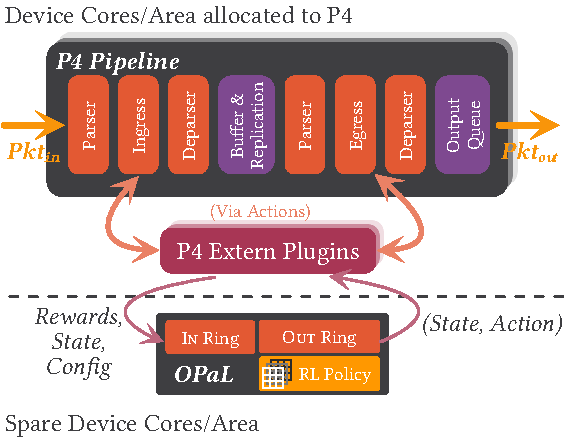
\includegraphics[keepaspectratio, width=0.85\linewidth]{diagrams/opal/arch-with-p4}
	\caption[\approachshort{}'s off-path interaction model with respect to a co-hosted P4 dataplane.]{SmartNIC-type \gls{acr:pdp} devices typically implement a target dataplane design by mapping the processing pipeline across one or more cores of \glspl{acr:fu}. Such devices are well-suited to this; \glspl{acr:npu} or \glspl{acr:soc} such as Netronome NFPs often have spare cores which aren't dedicated to running the dataplane, while spare area on \glspl{acr:fpga} may be used to design arbitrary \glspl{acr:fu}. While additional compute resources can relax the timing constraints needed to hit line-rate throughput, to prevent packet stalls as required we must move long-running computations (i.e., \gls{acr:rl} inference and updates) to this auxiliary compute. P4 programs expose device-specific functionality through \texttt{extern}s, allowing any extra compute resources and \gls{acr:ipc} to be accessed from ingress and egress tables, thus providing asynchronous execution and fast transmission of P4-extracted state as needed.\label{fig:netro-arch}}
%	\approachshort{} brings low-latency, online reinforcement learning directly to the dataplane. SoC- and NetFPGA-based SmartNIC devices expose spare compute---making in-situ, asynchronous processing and learning possible alongside P4 dataplanes. Classical RL policy methods are the key to making this computationally feasible. ?? REDO
\end{figure}

%?? 
%
%?? need to scale w/ available compute resources.
%
%?? need to not stall.
%
%?? Old, salesman-y.

\approachshort{} is a general, task-independent framework for in-network, online training and execution of \emph{any reinforcement learning agent design} using classical methods.
\approachshort{} is agnostic to the meaning of state vectors it receives as inputs and the actions it produces, which are employed by other functional units or the dataplane.
However, in-NIC/in-network execution specifically benefits packet-, flow-, and network-level learning, control, and optimisation tasks.
\approachshort{} meets the above goals by operating as a system which exists \emph{in parallel} to a co-hosted P4 dataplane.
\Cref{fig:netro-arch} describes and demonstrates the requisite interaction model; state extraction (i.e., flow telemetry collection and processing) occurs in the ingress and egress \glspl{acr:mat} of the P4 dataplane.
The packet pipeline of a P4 dataplane then communicates with \approachshort{} via \texttt{extern} plugins using \inring{} (state, configuration) messages to reconfigure the agent or request inference, and \outring{} (action) messages which carry output state-action pairs for the environment to make use of.
The protocol formats of these messages are explained below.
To deploy this design, we require a platform-specific implementation of \approachshort{} itself and the \inring{}/\outring{} ring interaction mechanisms---exploiting how SmartNIC devices often expose general-purpose compute.
As many of these devices have engineering and development histories which predate P4, such general compute beyond the P4 \gls{acr:psa}'s limits~\parencite{p4-psa} is surprisingly common.
This then provides path-adjacent, on-chip \gls{acr:rl} in the dataplane.

\approachshort{} itself runs on one or more cores of a SmartNIC to convert state measurements of a known size from the environment into a stream of actions using a stored policy.
I discuss how it scales with additional compute as part of \cref{sec:opal-algorithm}.
%As an example, this might be to map flow state and performance measurements into a queueing priority for future packets from that flow, or to compute and apply a rate limit to preserve quality of service.
These dedicated cores are then responsible for processing requests, computing actions, and updating the underlying policy in real time.
Combined with reward measurements, this policy can then be updated or trained from scratch entirely on the \gls{acr:nic}, acting as a fully online \gls{acr:rl} agent.
An input state vector \emph{always} induces an action and, if online learning is desired, updates the policy using either an included reward or one retrieved from memory according to a key placed alongside the state.
This allows for simultaneous control and learning over independent systems by the same agent (i.e., optimising several flows with their own reward measures, such as \gls{acr:ddos} mitigation in an \gls{acr:as} where each next-hop \gls{acr:as} might have their own health metric).
Configuration messages may be provided over either the data or control-planes, where the P4 control plane may be used to provide access control over which machines or ports may send such commands.

%?? How does this meet the above requirements?
By executing on spare compute units, this design prevents packet stalling as required by moving longer-running compute out of the packet path, and can scale with cores made available at compile-time to improve latency and throughput.
By operating as closely as possible to the P4 pipeline, \approachshort{} uses and learns from per-packet state with minimal added latency (avoiding \gls{acr:pcie} transfers and batching as required), while imposing minimal impact on carried traffic for both bump-in-the-wire deployments and at end-points.
Moreover, the presence of the P4 dataplane allows easier inclusion of existing P4 traffic measurement and state extraction techniques, such as those covered in \cref{chap:nets}.


%unused device resources beyond the P4-PSA spec \emph{can and should be used} to drive asynchronous environmental control

%\Cref{fig:netro-arch,fig:single-and-parallel} outline our design and implementation on Netronome SmartNIC hardware in pursuit of this goal: unused device resources beyond the P4-PSA spec \emph{can and should be used} to drive asynchronous environmental control.
%We explain relevant NFP architectural details later in \cref{sec:netronome-platform-fundamentals}.
%\approachshort{} communicates with the packet pipeline of a P4 dataplane via \texttt{extern} plugins using \inring{} (state, configuration) and \outring{} (action) messages (\cref{fig:netro-arch}).
%Internally, \approachshort{} either has all its cores act independently (\cref{fig:single-and-parallel:single}) or cooperate to solve each task (\cref{fig:single-and-parallel:parallel})---with different latency-throughput benefits (\cref{sec:action-and-update-computation}).
%We open-source our firmware and control programs for the benefit of the community.
%Moving beyond the Netronome platform, we describe how our architecture may be adapted and improved on by bespoke hardware or FPGA-based deployment.

%However, high-speed data networks impose inviolable per-packet deadlines.

%To protect traffic throughput and allow effective deployment in as many environments as possible, \approachshort{} places RL execution on-chip, \emph{but off the main packet path}, communicating and running parallel to the main P4 dataplane.
%As shown in \cref{fig:netro-arch}, this asynchrony allows coexistence with P4 programs, and imposes minimal impact on carried traffic for both bump-in-the-wire deployments and at end-points.
%For instance, in the default deployment of a P4 packet processing pipeline on Netronome NFP chips several cores go unused (as does spare area on an FPGA design), making this paradigm possible.

\paragraph{Message formats.}
?? Properly explain state/trace selection

\begin{minted}{rust}
pub enum HiThere {
    A(),
    B(),
}

let ggg = 0;
\end{minted}

\subsection{Data Format}\label{sec:opal-data-format}
%?? data format selection vs alternatives
To implement online learning such as in \gls{acr:rl}, we require a data type which allows us to perform numerical computation without an \gls{acr:fpu}---principally, to compute the values in action preference lists.
Moreover, to achieve online learning we require a format which is both fast to work with (to minimise processing latencies), and suited to represent gradients and temporal difference values i.e., incremental changes to stored policy weights.
Recalling the discussion in \cref{sec:numerical-representations-for-embedded-ml}, we employ \emph{fixed-point arithmetic}; it offers both the versatility needed to be easily reconfigurable, and it maps simply to \gls{acr:alu} operations.
For instance, only multiplications and additions require additional bitshifts for base pre-/post-conversion.\sidenote{Depending on system design, as with integers (hyper-)parameters used only in divisions can be replaced with right bitshift counts if we restrict their allowed values to negative powers of 2. This comes at the cost of system flexibility, and as such I don't make use of this possibility in \approachshort{}'s implementation.}

%?? Hence not binarised repr.
%?? Can choose bits allocated to fraction at runtime, overall bits at compile.
%?? Mention memory benefits.

From a configurability perspective, the number of fractional bits in a $Q$ number can be easily changed at runtime.
Naturally, this has no effect on overall latency and throughput of fixed-point arithmetic, but is a useful characteristic for being able to deploy different \gls{acr:rl} agents to the same hardware without invoking more costly firmware or \gls{acr:fpga} design installation.
If this is fixed at the same setting for all values used, then we needn't tag individual $Q$ numbers with information about their base, saving memory.
The bit width of the numbers themselves (i.e., $k$) may be changed only at compile time in many cases, particularly as SmartNICs often lack dynamic memory management in their native non-P4 programming environments.
Lower choices of $k$ sacrifice numeric range, but allow policies and data to occupy less memory---allowing fairer resource use versus other dataplane programs---and thus occupy less memory bandwidth in data transfers.
Alternately, larger policies may be stored in the same memory bounds (potentially enabling the solution of more complex problems).

Although reduced width floating-point formats have seen good successes in both inference and training on other resource-constrained devices, these require specialised \gls{acr:fpu} implementations.
This is naturally at odds with the design and goals of \gls{acr:pdp} hardware, and beyond \gls{acr:fpga} designs such a data format would be infeasible.
Software floating-point emulation has historically required \qtyrange{10}{30}{\times} more cycles to perform compared to hardware \glspl{acr:fpu}~\parencite{DBLP:conf/arith/IordacheT03}, which is incompatible with our need for low-latency and high-throughput processing.
While the added dynamic range would be useful in this application, performance is a primary goal.

\gls{acr:pdp} hardware excels in matching behaviours to network packets using \glspl{acr:mat}, potentially giving us a high-performance method to apply actions into the network.
However, directly modifying these match tables from within the device itself is neither feasible nor safe.
On Netronome NFP hardware in particular, rule updates \emph{must} be applied by the co-hosted controller machine, as tables are reliant on the optimised DCFL~\parencite{DBLP:conf/infocom/TaylorT05} data format.
In addition to the prohibitive complexity of building this data structure on-device, its construction requires knowledge of the entire rule set (and cannot be incrementally updated).

\subsection{Algorithm}\label{sec:opal-algorithm}

?? algo selection

?? Need to discuss compute strategies; coop vs parallel here.

?? Note worth having here (and the paper itself): past `parallel Sarsa'~\parencite{DBLP:conf/aamas/GroundsK07} means `learning from parallel agents' traces': OPaL enables this too to some extent!

?? old, salesman-y
To enable \emph{online in-NIC learning}, we return to \emph{classical} RL methods and models.
In particular, we focus on tile-coding with one-step temporal-difference learning algorithms such as Sarsa.
%These choices have important benefits for in-NIC execution.
These functions do not require batches of inputs to learn in a stable way, negating the memory needed to store experience replays, and have simple update and inference logic.
Finally, the choice of single-step algorithms (as opposed to $n$-step or Monte Carlo methods) bounds the amount of per-trace state required for online learning to just the last state-action pair, safeguarding the limited memory of the target devices.

\begin{figure}
	\centering
	\resizebox{0.67\linewidth}{!}{
		\begin{tikzpicture}
	\node at (0,0) {
		\begin{tikzpicture}
			\draw[step=0.5cm,color=uofgcobalt,opacity=0.7,shift={(0,0)},label=above:{Tiling 0}] (-0.5,-0.5) grid (1,1);
			\fill[uofgcobalt,opacity=0.5] (0.5,-0.5) rectangle (1,0);
			\node[color=uofgcobalt] (t1g) at (0,1.2) {\footnotesize Tiling 1};
			
			\draw[step=0.5cm,color=uofgpumpkin,opacity=0.9,shift={(0.25,-0.25)},label=above:{Tiling 1}] (-0.5,-0.5) grid (1,1);
			\fill[uofgpumpkin,opacity=0.5,shift={(0.25,-0.25)}] (0,0) rectangle (0.5,0.5);
			\node[color=uofgpumpkin!50!uofgrust] (t2g) at (0.25,-0.95) {\footnotesize Tiling 2};
			
			\node[circle, black, draw,
			fill, radius=0.5pt, inner sep=0pt,minimum size=1.5pt, label=above:{$s$}] at (0.625,-0.125) {};
			%			\filldraw (0.625,-0.125) circle[radius=1.5pt,label=above:{$s$}];
			
			\draw[->] (-0.25,-0.5)--(-0.25,0.85);
			\draw[->] (-0.25,-0.5)--(1.1,-0.5);
			
			\node at (1,-0.7) {\footnotesize 1};
			\node at (-0.4,0.75) {\footnotesize 1};
			\node at (-0.35,-0.6) {\footnotesize 0};
		\end{tikzpicture}
	};
	
	\node (policy-head) at (2.5,1.2) {Policy};
	\draw[color=uofgcobalt,opacity=0.7] (2,0) rectangle ++(2,1) node[pos=.5] (t1p) {Tiling 1};
	\fill[uofgcobalt,opacity=0.25] (3.33,0) rectangle ++(0.67,0.33);
	
	\draw[color=uofgpumpkin,opacity=0.9] (2,-1) rectangle ++(2,1) node[pos=.5] (t2p) {Tiling 2};
	\fill[uofgpumpkin,opacity=0.25] (2.67,-0.67) rectangle ++(0.67,0.33);
	
	\draw (2,-2) rectangle ++(2,1) node[pos=.5] (tdot) {$\cdots$};
	
	\draw [->,color=uofgcobalt, bend left] (t1g) to (t1p.west);
	\draw [->,color=uofgpumpkin, bend right] (t2g) to (t2p.west);
	
	\node (act-list) at (1,-2.5) {$\mathbf{a}=\left[ \cdots \right]$};
	
	\draw [->, bend right] (t1p.west) to (act-list);
	\draw [->, bend right] (t2p.west) to (act-list);
	\draw [->, bend right] (tdot.west) to (act-list);
\end{tikzpicture}
	}
	\caption[A visualisation of how tile-coding can be split into subtasks as a map-reduce problem.]{Tile-coded function approximation can be considered as a map-reduce problem during both the inference and update steps. Action preferences are aggregated from \emph{disjoint} tile queries, where each tile hit contains a list of action values to add to $\mathbf{a}$. Checking or updating each tiling is thus a separate task. As all candidate lists are disjoint between tasks, updating hit tiles requires no control over concurrent accesses---furthermore, it requires no final aggregation step.\label{fig:opal-par-tilecode}}
\end{figure}

?? proof of map-reduceness?

aa

\begin{algorithm}
	\caption{ParSa---\emph{Par}allel \emph{Sa}rsa\label{alg:parsa}}
	\SetKw{Let}{let}
	\SetKw{Enum}{enum}
	\SetKw{In}{in}
	\SetKw{Await}{await}
	\SetKw{Const}{const}
	\SetKwProg{parsa}{Function \emph{ParSa}}{}{end}
	\SetKwProg{control}{Function \emph{Ctl}}{}{end}
	\SetKwProg{minion}{Function \emph{Minion}}{}{end}
	\SetKwProg{tilecode}{Function \emph{TileCode}}{}{end}
	
	\tcc{Given message passing mechanisms \emph{scatter} and \emph{recv}, quantised arithmetic functions $Q_\mathit{mul}$ and TileCode, and omitting schedule/config/precache updates.}
	\tcc{\emph{cfg}.$\alpha$, \emph{cfg}.$\gamma$ are hyperparameters affecting the significance of each update and the degree of forward-planning, respectively.}
	
	\Enum Par \{ Act(\emph{state}), Upd(\emph{delta, action, state}) \}\;
	\Const \emph{cfg, policy} = /* ... */\;
	
	\Let \emph{values}: [AtomicI32; \emph{cfg.n\_actions}] = \{0\}\;
	\Let \emph{acks}: AtomicI32 = 0\;
	\parsa{id, schedule}{
		\uIf{id==0}{
			\ForAll{state\_pkt \In \inring{}}{
				Ctl(\emph{state\_pkt})\;
			}
		}
		\Else{
			\While{true}{Minion(\emph{schedule}[$\mathit{id}- 1$], recv())\;}
		}
	}

	\control{state}{
		\emph{values, acks} = \{0\}, scatter(Par::Act(\emph{state}))\;
		acquire slot for \outring, copy \emph{state} into slot\;
		\Await acks == \emph{cfg.n\_minions}\;
		\Let \emph{action} = argmax(\emph{values})\;
		write \emph{action} into \outring{} slot, enqueue\;
		\If{cfg.online}{
			\Let \emph{((l\_state, l\_act, l\_val), found\_s)} = \emph{cfg}.lookup\_state\_from\_key(\emph{state})\;
			\Let \emph{(reward, found\_r)} = \emph{cfg}.lookup\_reward\_from\_key(\emph{state})\;
			\If{found\_s \&\& found\_r}{
				\Let $\delta_t$ = $\mathit{reward} + Q_\mathit{mul}$(\emph{cfg}.$\gamma$, \emph{values}[\emph{action}]) $-$ \emph{l\_val}\;
				$\delta_t$ = $Q_\mathit{mul}$(\emph{cfg}.$\alpha$, $\delta_t$)\;
				\emph{acks} = 0, scatter(Par::Upd($\delta_t$, \emph{l\_act}, \emph{l\_state}))\;
				\Await acks == \emph{cfg.n\_minions}\;
			}
			\emph{cfg}.store\_state(\emph{state}, \emph{action}, \emph{values}[\emph{action}])\;
		}
	}

	\minion{tasks, msg}{
		\Switch{msg}{
		\uCase{Par::Act(\emph{s})}{
			\ForAll{task \In tasks}{
				\Let \emph{hit} = TileCode(\emph{s}, \emph{task})\;
				\For{i \In [0..cfg.n\_actions)}{
					\emph{values}[\emph{i}].atomic\_add(\emph{policy}[\emph{hit}][\emph{i}])\;
				}
			}
		}
		\uCase{Par::Upd($\delta$, \emph{a}, \emph{s})}{
			\ForAll{task \In tasks}{
				\Let \emph{hit} = TileCode(\emph{s}, \emph{task})\;
				\emph{policy}[\emph{hit}][\emph{a}] += $\delta$\;
			}
		}
		}
		\emph{acks}.atomic\_add(1)\;
	}

%	\tilecode{state, task}{
%		\Let \emph{hit} = \emph{cfg}.get\_task(task)\;
%	}
\end{algorithm}
